\documentclass[12pt,letterpaper]{article}

% just for the example
\usepackage{lipsum}
\usepackage{url}
% Set margins to 1.5in
\usepackage[margin=1.5in]{geometry}

% for graphics
\usepackage{graphicx}
\graphicspath{{./figures/project-principles/}}

% for crimson text
\usepackage{crimson}
\usepackage[T1]{fontenc}

% setup parameter indentation
\setlength{\parindent}{0pt}
\setlength{\parskip}{6pt}

% for 1.15 spacing between text
\renewcommand{\baselinestretch}{1.15}

% For defining spacing between headers
\usepackage{titlesec}
% Level 1
\titleformat{\section}
  {\normalfont\fontsize{18}{0}\bfseries}{\thesection}{1em}{}
% Level 2
\titleformat{\subsection}
  {\normalfont\fontsize{14}{0}\bfseries}{\thesection}{1em}{}
% Level 3
\titleformat{\subsubsection}
  {\normalfont\fontsize{12}{0}\bfseries}{\thesection}{1em}{}
% Level 4
\titleformat{\paragraph}
  {\normalfont\fontsize{12}{0}\bfseries\itshape}{\theparagraph}{1em}{}
% Level 5
\titleformat{\subparagraph}
  {\normalfont\fontsize{12}{0}\itshape}{\theparagraph}{1em}{}
% Level 6
\makeatletter
\newcounter{subsubparagraph}[subparagraph]
\renewcommand\thesubsubparagraph{%
  \thesubparagraph.\@arabic\c@subsubparagraph}
\newcommand\subsubparagraph{%
  \@startsection{subsubparagraph}    % counter
    {6}                              % level
    {\parindent}                     % indent
    {12pt} % beforeskip
    {6pt}                           % afterskip
    {\normalfont\fontsize{12}{0}}}
\newcommand\l@subsubparagraph{\@dottedtocline{6}{10em}{5em}}
\newcommand{\subsubparagraphmark}[1]{}
\makeatother
\titlespacing*{\section}{0pt}{12pt}{6pt}
\titlespacing*{\subsection}{0pt}{12pt}{6pt}
\titlespacing*{\subsubsection}{0pt}{12pt}{6pt}
\titlespacing*{\paragraph}{0pt}{12pt}{6pt}
\titlespacing*{\subparagraph}{0pt}{12pt}{6pt}
\titlespacing*{\subsubparagraph}{0pt}{12pt}{6pt}

% Set caption to correct size and location
\usepackage[tableposition=top, figureposition=bottom, font=footnotesize, labelfont=bf]{caption}

% set page number location
\usepackage{fancyhdr}
\fancyhf{} % clear all header and footers
\renewcommand{\headrulewidth}{0pt} % remove the header rule
\rhead{\thepage}
\pagestyle{fancy}

% Overwrite Title
\makeatletter
\renewcommand{\maketitle}{\bgroup
   \begin{center}
   \textbf{{\fontsize{18pt}{20}\selectfont \@title}}\\
   \vspace{10pt}
   {\fontsize{12pt}{0}\selectfont \@author} 
   \end{center}
}
\makeatother

% Used for Tables and Figures
\usepackage{float}

% For using lists
\usepackage{enumitem}

% For using APA Citation format
\usepackage{apacite}

% Custom Quote
\newenvironment{myquote}[1]%
  {\list{}{\leftmargin=#1\rightmargin=#1}\item[]}%
  {\endlist}
  
% Create Abstract 
\renewenvironment{abstract}
{\vspace*{-.5in}\fontsize{12pt}{12}\begin{myquote}{.5in}
\noindent \par{\bfseries \abstractname.}}
{\medskip\noindent
\end{myquote}
}

\begin{document}

% Set Title, Author, and email
\title{Project - Principles\\Analysis of JupyterLab Interface}
\author{Snejana Shegheva \\ sshegheva3@gatech.edu}

\maketitle
\thispagestyle{fancy}

\begin{abstract}
JupyterLab is a web-based interface for Project Jupyter that provides an interactive and reproducible computing platform\footnote{https://github.com/jupyterlab/jupyterlab}. In this project, we evaluate the interaction with Documents and Kernels, specifically with the Notebook plugin that serves an observable list of cells containing code, markdown, or raw data.  
\end{abstract}

\subsection*{Heuristic Evaluation}
Figure~\ref{fig::1} shows an example of my current JupyterLab workspace, that include a file navigation section, interactive notebook area, additional consoles, and many other things that the platform provides. As a development environment, JupyterLab allows access to terminals, file viewers, notebooks, text editors - all from one place, which I personally find very convenient. With a rapid growth of data science and machine learning, Jupyter Notebooks have become a standard for creating reproducible computational narratives \cite{blog:jupyter}. 

\textbf{What works well}. Its most attractive feature - interactivity - thrives in both gulfs: \textit{execution} and \textit{evaluation}. In the former case, the cells provide a clear indication for where text/code should be entered. In the later case, executing a cell yields immediate feedback that allows user assessing how well their intentions have been met. Cells are viewed as building blocks, and as such can be re-arranged using a \textit{direct manipulation} via drag-n-drop functionality. User is engaged in the process of interacting with the interface by 1) planning the action, for example, hovering over the cell that needs to be moved; 2) grabbing the cell and dragging it over the area that specifies the new location; 3) performing the cell move operation by releasing the hold. The interface is so intuitive largely due to the tight relationships between two gulfs. As the user is performing the action of re-arrangement, the system provides a "hint" in form of target line for where the new cell would land before the action is complete. Therefore, the goal can be accomplished more accurately and more efficiently with means to see and interpret the actions and necessary adjustments.      

\begin{figure}[h]
\centering
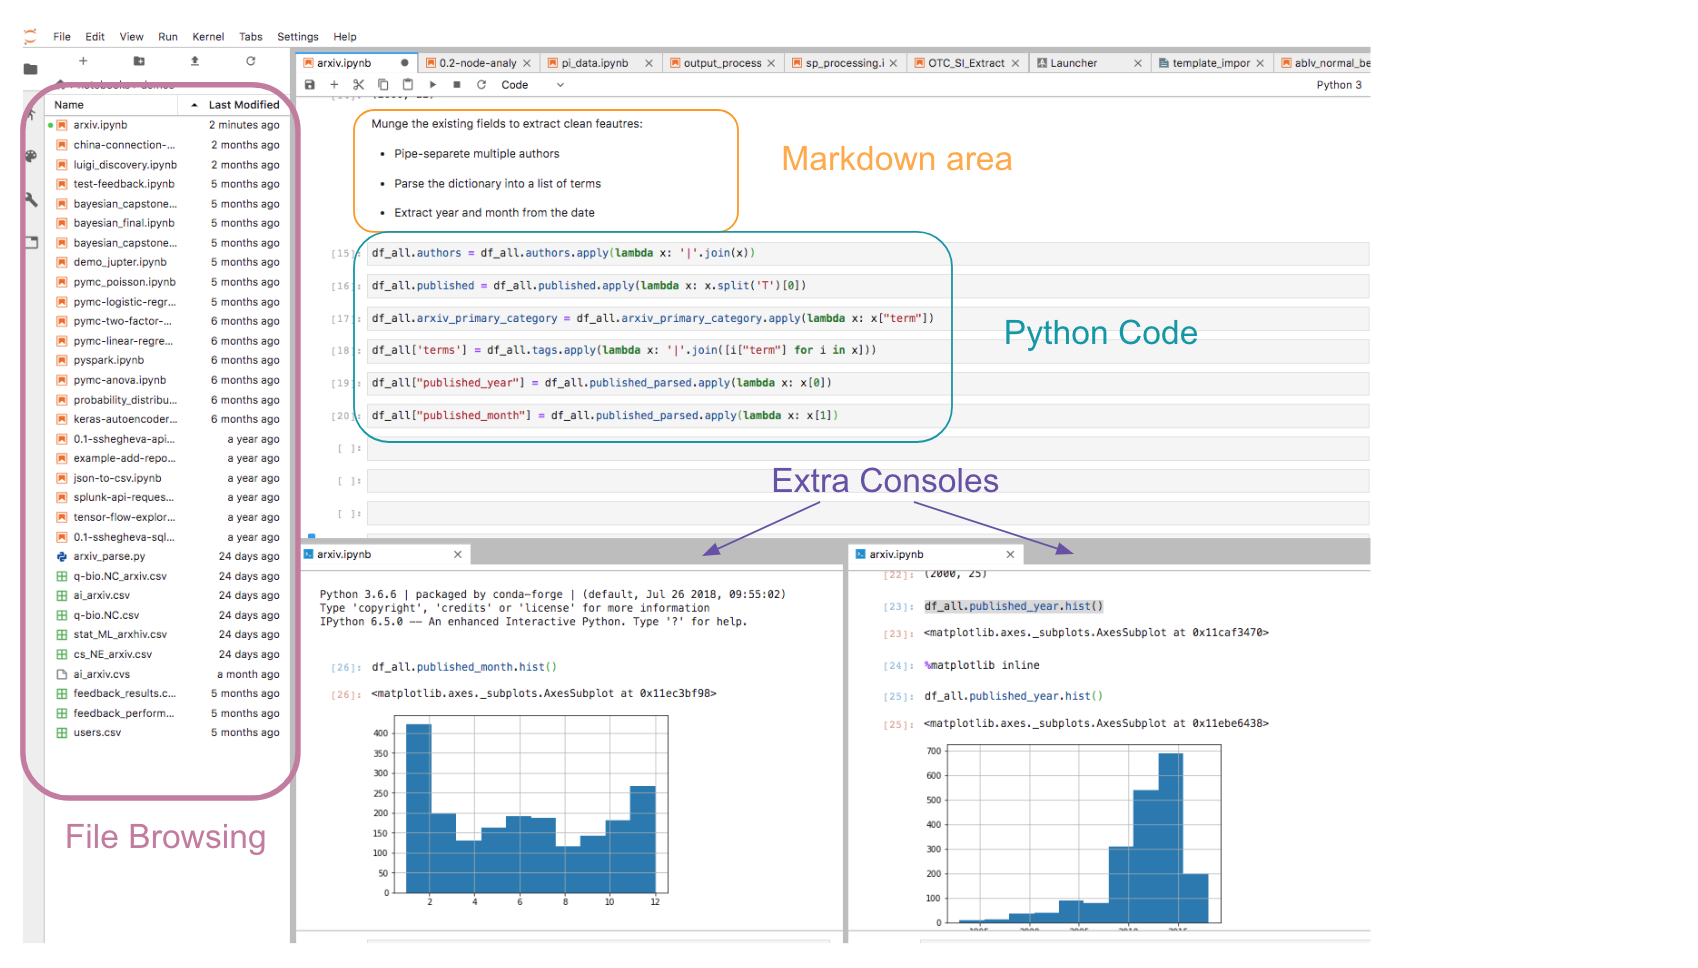
\includegraphics[scale=.5]{figures/project-principles/jupyter.png}
\caption{An example of JupyterLab Workspace.}
\label{fig::1}
\end{figure}

\textbf{What doesn't works well}.

\iffalse
2.1 Introduction to Principles
2.2 Feedback Cycles
2.3 Direct Manipulation and Invisible Interfaces
2.4 Human Abilities
2.5 Design Principles and Heuristics
2.6 Mental Models and Representations
2.7 Task Analysis
2.8 Distributed Cognition
2.9 Interfaces and Politics
2.10 Conclusion to Principles

First, perform a heuristic evaluation using the principles from Unit 2 on the interface as it currently exists. Answer the questions: what works well? What makes it work well? What doesn’t work well? Why doesn’t it work well? Make sure to address all these: even the worst interfaces usually have some things that work well. If you can’t think of any good things to say about the interface, select a different one: redesigning an interface with no positive elements at all would be too easy!

In writing this evaluation, it is critical that you ground your critiques in terms of the principles you have learned in Unit 2, both conceptually and using the same vocabulary. Your critique will primarily be evaluated based on how well it grounds its praise and criticism in the principles covered in Unit 2, and how accurately it leverages these principles. We would expect any strong answer to use at least five principles covered in Unit 2, where a ‘Principle’ can be nearly any topic from the unit, including any of the design principles, ideas like expert blindspot and learning curves, and concepts like gulfs of execution and evaluation. However, you are not limited to five principles, nor is five principles automatically sufficient if the individual principles are not leveraged with sufficient depth.
\fi

\subsection*{Interface Redesign}
Second, based on your evaluation, redesign the interface. If it’s a visual interface (such as a mobile app, visual wearable interface, or traditional desktop application), supply visual mock-ups of the potential redesign. If it’s a physical interface, supply a sketch or similar representation of the altered interface. If it’s an interface that cannot be provided in a 2D visual form like a haptic, auditory, or virtual reality interface, describe the redesign in words using diagrams wherever possible. Your redesign can contain textual annotations or rely on text if it is non-visual, but the text should merely explain the redesigned interface, not justify it.

\subsection*{Interface Justification}
Third, justify the redesigned interface. Describe how your redesigned interface addresses the criticisms from the first section, while preserving the positive elements of the original interface. Again, make sure to put your justification in terms of the principles covered in Unit 2, both conceptually and using the same vocabulary. You need not focus on the same principles covered in the previous section; you may, for example, leverage a particular principle to improve the interface even if it wasn’t explicitly violating that principle in the first place.

\bibliographystyle{apacite} 
\bibliography{bibtemp}

\end{document}
